% CREATED BY DAVID FRISK, 2016
\chapter{Results}
\todo{By results, do we limit ourselves to the usability tests? If not we need to change this opening text. /H}
Results can be presented in different ways. One way would be to describe the usability tests in detail, and another way would be to only summarize the results in table. 
By describing all usability tests in detail, it would be hard to get a good overall view of the findings. Focusing more on something also means focusing less on something 
else, and there are other parts of the documentation that deserve that attention more. It would therefore not be ideal to do lengthy elaborations on each teaching material.
On the flip side, only giving a summary on the findings would leave out describing the crucial process. The process mainly includes:
\begin{enumerate}
	\item Performing a usability test
	\item Identifying what can be learned from the data
	\item Figuring out how the particular teaching material can be improved from the data
	\item Revising the teaching material (preferably in an effective manner)
\end{enumerate}
The ideal way of delivering the results should entail a comporomise between these two extremes. The finding has therefore been divided into a sample case and a summary.
The sample case describes a teaching material thouroughly, delving into details of the process and findings, exemplifying the usability testing process. 


%

\section{Summary of usability test results}


\begin{table}[H]
\centering
\caption{Summary of all usability tests of the study}
\begin{tabular}{lll} \hline\hline
  Date for test & Material that was tested & Test subject \\ \hline
  2018-04-24 & Mönster och talföljder - Pascals triangel ur slantsingling & A30T2 \\ \hline
  2018-04-30 & Nätverk - insamling av data & B25S \\ \hline
  2018-05-03 & Vad ska lotten kosta? & C37T3 \\ \hline
  2018-05-09 & Konsten att bestämma arean & D33T6 \\ \hline
  2018-05-09 & Område statistik & E38T4 \\ \hline
  2018-05-14 & Modellering & F50T30 \\ \hline
  2018-05-14 & Nätverk - insamling av data & F50T30 \\ \hline
  2018-05-24 & Mönster och talföljder - Pascals triangel ur slantsingling & G26T2 \\ \hline
  2018-05-24 & Den dolda och tvetydiga matematiken & G26T2 \\ \hline
  2018-05-30 & Den dolda och tvetydiga matematiken & H27S1 \\ \hline
  2018-06-12 & Den dolda och tvetydiga matematiken & I30T1
  \\ \hline\hline
\end{tabular}
\end{table}

\section{Sample case 1. Kleinmaterial: Nätverk}
Each teaching material tested has a different story to tell. Keep in mind that some of the content of the steps below are common to all teaching materials tested, while some are specific to the particular teaching material.

\subsection{The preexisting work}
The sample teaching material was produced by a team at Kleindagarna. These consisted of a handful of teachers, a subject expert and a Klein-representative. When the workshop at Kleindagarna was over, the teaching material was published on Kleindagarna's website. 

\subsection{Usability test I}
The first usability test was performed by one of the authors of this report on the other author. As this was the second ever usability test performed, the intention was primarily to identify what to take into account for future usability testing and to identify the possibility of improving the usability testing methodology. The method consisted of following a script document on a computer including:
\begin{description}
    \item $\bullet$ A table made to be filled with personal information
    \item $\bullet$ A list of keywords and questions (manuscript) inspired by the usability test script created by Steve Krug.
\end{description}

\paragraph*{}
Results from this test included:
\begin{description}
    \item $\bullet$ Unclear if some tasks were meant to be executed by teacher or students.
    \item $\bullet$ The material expected the teacher to be very familiar with the subject, tackling advanced areas of mathematics with mostly bullet points, expecting the teacher to provide the explanation.
    \item $\bullet$ There was a concern on the material having too large scope. The material includes network theory, statistics, algorithms and data protection laws (GDPR), and aims to both explain and problematize all of these aspects.
\end{description}
\subsection{Revision of methodology}
After usability testing the teaching material, the authors identified that there was very limited information presented in the list of teaching materials on Kleindagarna's website. This made it difficult for the curious to know if the material was suitable for them. Because of that, a new list of teaching materials was compiled. This consisted of information not just what the subject of the material was, but also for what grade it was suited and a more detailed description of the teaching material.\\
After the usability test, a discussion arose on what type of material the revisions would be. Two suggested possibilities were documents (i.e. pdf- or odt-files) and presentations (e.g. pptx-files). A document would have the strength of being easily skimmed and modified. A presentation would have the strength of being a ready-made lesson material, with the potential of not requiring as much planning time. The discussion culminated in the decision to choose type on a case-by-case basis. Some factors to take into account when deciding on the type would be: results from usability tests, perceived intent of original creators and what form would be most suited for the particular teaching material.
\subsection{Watching the Klein-lecture}
Before designing a teaching material, the participators on Kleindagarna receive a lecture by the subject-expert. This lecture was recorded and confidentially shared online. Before revising the material, it was decided that it would be beneficial to watch this lecture, to learn more about the theory the material was based upon and what the creators intended the students would learn.
\subsection{Usability test II}
The same revision was tested again. The test subject this time was a Klein-representative that had been involved in the creation of the original teaching material. Testing teaching materials on a subject that was not a teacher in upper-secondary-school or a teacher student aiming to teach at upper-secondary-school was not the norm. One purpose of this was to analyze how rewarding usability testing non-intended subject could be. The test subject is also teaching mathematics on an upper-secondary-school level, but to post-secondary school students (one additional difference is that the pace of the courses are comparably higher than in upper-secondary-school). Results from this test included:
\begin{description}
    \item $\bullet$ The teaching material wasn't considered complete by the creators.
    \item $\bullet$ The biggest remaining problem of the material design lies in a student activity where the class are to compile data to create a network. To be able to make the network and its analysis meaningful, it was suggested that the compiled data should be personal and able to lead to a finding. Ultimately, the activity asks for generated data, instead of personal, more valuable data. The reason for this is because no conceivable alternative could eliminate the risk that personal data could result in undesirable findings. For example if the data collected answers what students had lunch together, outcasts are visible in the finding.
\end{description}
\subsection{Revision of teaching material}
From the data collected, the following revisions were made:
A decision was made to revise the material in the form of a presentation. With the aim to offer a ready-made presentation with enough explanation of the required theory to be a desirable product. To realize this, changes were made to the structure and to content.
\subsubsection*{Structural changes}
\begin{description}
    \item $\bullet$ The separation of information to the teacher and the main presentation was improved by implementing tabs similar to how many websites function. This also clarified the structure to the user, enabling the user to quickly get an overview of the structure.
    \item $\bullet$ The presentation's first slides contains useful information targeted to a curious teacher including how to read the important presentation notes (as these consists of teacher instructions and explanations).
\end{description}
\subsubsection*{Content changes}
\begin{description}
    \item $\bullet$ As mentioned previously, the presentation contains teacher instructions and explanations in the form of presentation notes. These can be printed or read in the presentation program, and also viewed while presenting. This was previously missing from the teacher material, or carelessly intertwined with content that seemed to be aimed to students.
    \item $\bullet$ Activities were altered to be either less vague or more closely tied to what the students are expected to learn.
    \item $\bullet$ The content was modified to be easily understood and conveyed. An example of this was replacing the headings so that they describe their respective slide, instead of being named after the current 5E-phase.
\end{description}
\subsection{What was learned from this case?}
From this particular case, the following knowledge was obtained:
\begin{description}
    \item $\bullet$ Someone involved in the creation of a teaching material can have a very different experience and connection to the teaching material, than is conveyed to a reader. Maybe there's a part the creator is not satisfied with, but the reader might assume it is meant to be complete and only understand it as poorly made. This exemplifies the flaws of one-way communication perfectly.
    \item $\bullet$ There needs to be a decision on how the teaching material is presented and what it aims to be. It can be everything from inspiring reading material to a documentary. It was decided that the two types of material explored in this thesis would be \textit{document with proposed lesson plan} and \textit{ready-made presentation}.
\end{description}

\section{Sample case 2. Kleinmaterial: Vanliga missuppfattningar}

\subsection{The preexisting work}

Just like the Sample case 1, the sample teaching material was produced by a team at Kleindagarna. See Sample case 1, section [REFERENS: Sample case 1], for more information.

\subsection{Usability test I}

[TODO]

\section{The materials list}

The original list of materials was remade from scratch and revised continuously after feedback from the usability tests. It proved useful as a way to study how the teachers picked their materials, and what information they want when doing so.

[Blah more intro blah]

\subsection{Revisions of the materials list}

\begin{figure}[H]
\centering
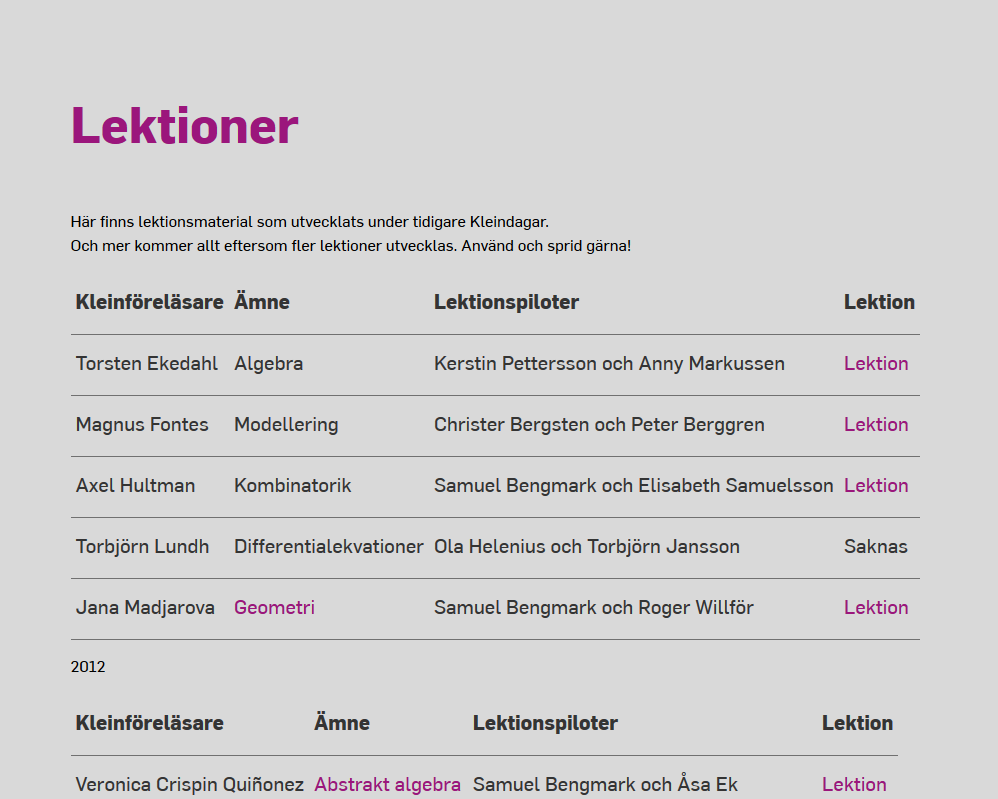
\includegraphics[width=\linewidth]{figure/screenshot_materiallista_kleindagarna.png}
\caption{The original list of materials on Kleindagarna's official website [SOURCE].}
\end{figure}

Note that the design of Kleindagarna's list of materials changed in the middle of the thesis. Most of the information in the list remained the same, but colors and fonts changed. A screenshot of the list before Kleindagarna's change wasn't made and thus the exact changes were lost. The first and second thesis-revisions of the list were made before Kleindagarna made changes to their list.

\begin{figure}[H]
\centering
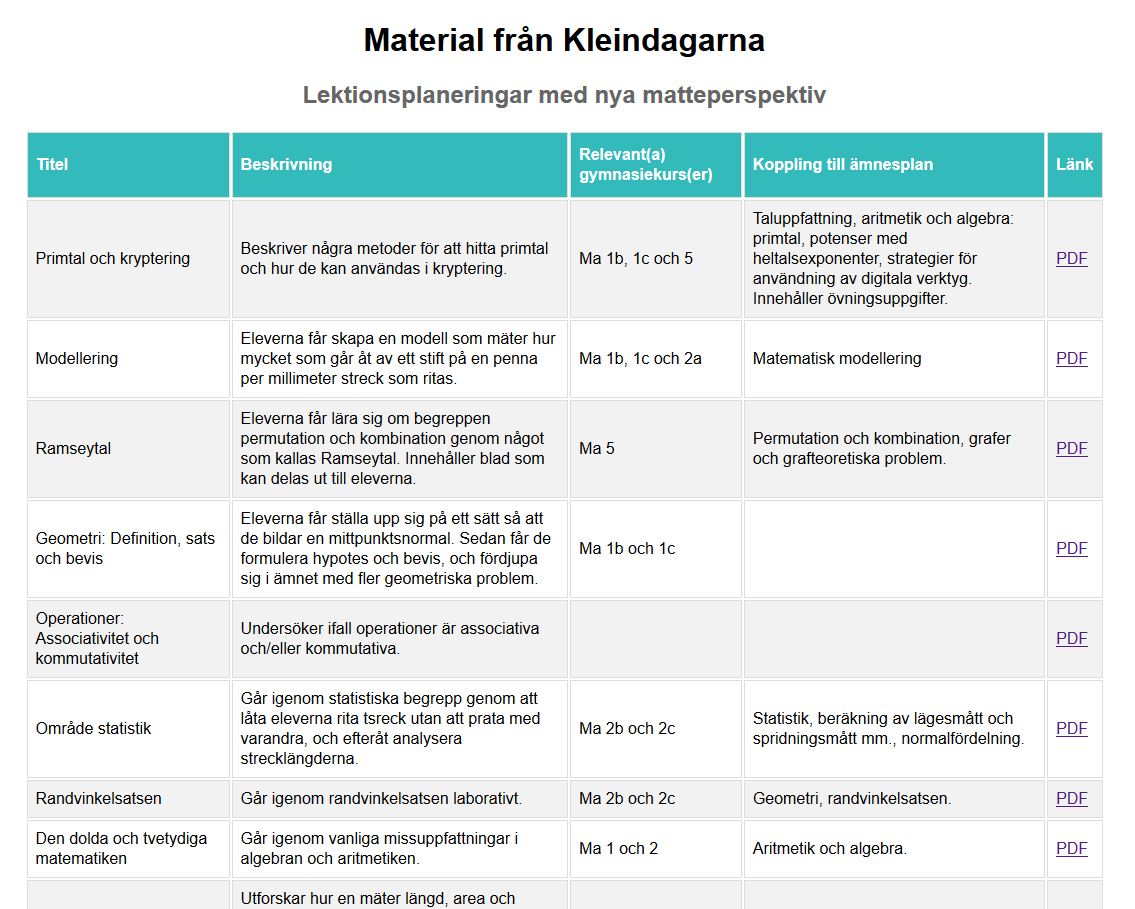
\includegraphics[width=\linewidth]{figure/screenshot_materiallista_revision_2.png}
\caption{The second revision of the list of materials, based on Kleindagarna's original [FIGURE REFERENCE?].}
\end{figure}

Comparing the original list with the revised list, a couple of things were changed:
\begin{enumerate}
	\item A tagline was added under the title: "Lektionsplaneringar med nya matteperspektiv" in Swedish, or "Lesson plans with new mathematical perspectives" in English. This was meant to change the expectations of the teachers looking through the list, so they knew the materials were about mathematics, and that they had innovative perspectives on mathematics rather than remaking typical maths lesson materials.
	\item A description was added for every material due to teachers expressing during the tests that they wanted to know more about the material they were going to choose. The descriptions were originally taken directly from the materials and slightly reworked, leading to some materials lacking a description due to not having one in the material itself. This further lead to teachers ignoring the materials that were lacking a description during some tests. Thus, descriptions were added to all the materials.
	\item The "Lektionspiloter" and "Kleinföreläsare" parts of the list were removed since few of the test subjects would understand what it was or know the people by name, and more space was needed for other information.
	\item "Relevant(a) gymnasiekurs(er)", in English "Revelant secondary school course(s)", were added due to them existing in most of the materials themselves, and thus easily added into the list. Likewise, "Koppling till ämnesplan", "Connection to the subject curriculum" in English, was added in the same way, also replacing "Ämne" in the original list..
	\item A title was added to every material in the list to make the materials more scannable instead of having to read the whole description to understand the general idea of the material.
\end{enumerate}

\subsection{Results from studying how teachers chose their materials}

[TODO]

\section{General perspective: Things that were learned from all the usability tests}
The previous usability test cases in this chapter described how results were produced from a couple of specific tests. In a similar manner, more results were produced by going through the tests one by one and summarizing the findings from a holistic perspective - in other words, by comparing the tests next to each other. Below are some findings from this general analysis.

\subsection{Comparisons between the teachers' typical lessons}
As described earlier [REFERENS? GÖR VI DETTA I METODKAPITLET?], part of the usability test consisted of asking the teachers what their typical lesson looked like. Here are some comparisons between these typical lessons.

\begin{itemize}
  \item Pretty much every teacher used a combination of lectures in group and individual student exercises, even if their lesson lengths and structures were different. [...FORTSÄTT?]
\end{itemize}

\subsection{Making the material intuitive for different behaviours is important}
Because of the difference in how teachers read a material, where one might instantly read the material in-depth and the other might just scroll down while scanning it, having a material be intuitive at first glance is a good thing. Some materials took the teachers a while to understand, which could have been rectified through a more clear structure and by following typical patterns that the teachers are used to. One pattern that was asked for directly in two of the usability tests [REFERENSER: UBH,UBI] was to have an introductory text, which was lacking for the specific material that was tested. At the same time, in one of the tests [REFERENS: UBA] the teacher completely ignored the introduction to make sense of the material's content by itself. In either case, the material should ideally be clear to understand for both types of material reading behaviours.

\subsection{Having student handouts as part of a material is appreciated}
All materials didn't have parts that could be handed out to students, such as a list of exercises. However, many teachers seemed to appreciate such "handouts", or ask for them when they were missing. For example, one teacher wanted a handout for the student that explained a difficult word that they hadn't encountered before [REFERENS: UBD]. Another teacher said that they could use a list of exercises by itself without following the exact lesson plan, which shows that exercises as a part of a material can improve the adaptability of the material. In contrast to this, one teacher expressed that materials can also work as a source of inspiration rather than something concrete and finished as a handout or a finished lesson plan. An important aspect of both of these materials, the "concrete handout" and the "source of inspiration", is the amount of work that these different types require for adaption into a real lesson: The handout can be printed and handed out directly, while the inspiration has to be reworked into a new material.

\subsection{Accounting for teachers' and students' previous knowledge}
A common problem among many materials was the teacher's lack of previous knowledge about the subject that the material presented. The most common and concrete problem that appeared was when new vocabulary was used, such as RSA [REFERENS: UBC,UBH] and Dido's problem [REFERENS: UBH]. There was also an issue with one teacher not feeling competent enough to teach a subject that a material covers [REFERENS: UBE]. In contrast, another teacher expressed that a material could be explored together with the students when the teacher didn't know everything about it either [REFERENS: UBC]. Similarly, some materials seemed too difficult for certain teachers to use due to their students' lack of previous knowledge [REFERENS: UBD,UBE].

\subsection{Finding common usability problems}
In every test, at least one unclear explanation or structure, unanswered question, or other smaller, easily rectified usability problem was found. Thus, the usability tests proved effective in finding these problems. Examples of the problems found include:
\begin{itemize}
	\item No clear explanation about what part the student should do and what part the teacher should do during a lesson.
	\item A lack of description of the axes in a diagram.
	\item Mixed use of comma (,) and dot (.) as decimal separator.
	\item An undefined word that needed explanation (Galton board).
	\item Unclear use of the 5E-structure when it wasn't used as the teacher expected it to be used.
	\item Unclear whether "degrees" was referencing temperature, geometric angles, or "levels."
	\item Misunderstandings about what a list of exercises was, where the teacher described it simply as a "list" of unknown purpose.
	\item Instructions that required more explanation. In this case, the instructions merely showed a couple of numbers without describing what the numbers were for; "0,0,0,50...", where it was explaining a point system for gambling with dice.
\end{itemize}

Although many of these misconceptions were often understood by the test subject after a while, it often took a lot of time, and likely frustration, for them to figure it out.
